\documentclass[pdftex,12pt,a4paper]{report}

\usepackage[portuguese,english]{babel}
\usepackage[T1]{fontenc} 
\usepackage[table,xcdraw]{xcolor}
\usepackage[utf8]{inputenc}
\usepackage[pdftex]{graphicx}
\usepackage{minitoc}
\usepackage{hyperref}
\usepackage{indentfirst}
\usepackage[compact]{titlesec}
\usepackage{fancyhdr}
\usepackage{caption}
\usepackage{pgfplots}
\usepackage{pgfplotstable}
\usepackage{fixltx2e}
\usepackage{mathtools}
\usepackage{fancyhdr}
\usepackage{listings}
\usepackage{color}
\usepackage{sverb}
\usepackage[section]{placeins}
\usepackage{adjustbox}
\titleformat*{\subsubsection}{\itshape}


%Highlight
\newcommand{\shellcmd}[1]{\indent\indent\texttt{\footnotesize\# #1}\\}

\pagestyle{fancy}
\renewcommand*\thesection{\thechapter\arabic{section}}
\newcommand{\HRule}{\rule{\linewidth}{0.5mm}}
\begin{document}

\begin{titlepage}

\begin{center}


\includegraphics[width=0.15\textwidth]{./logo}\\[0.5cm]    

\textsc{\large Universidade de Aveiro \\[1cm]\large departamento de electrónica, telecomunicações e informática}\\[1cm]

\textsc{\large{1}\large - Desempenho e Dimensionamento de Redes\\[1cm]}

\HRule \\[0.5cm]
{ \huge \bfseries abs}\\[0.4cm]
{ \large \bfseries x}\\[0.4cm]
\HRule \\[1cm]

\textsc{\small{8240 - MESTRADO INTEGRADO EM ENGENHARIA DE COMPUTADORES E TELEMÁTICA}}\\[1cm]

\begin{minipage}{0.4\textwidth}

\begin{flushleft} \large
\href{mailto:rafael.ferreira@ua.pt}{António Rafael da \\ Costa Ferreira }
 \small{\\NMec: 67405}
\end{flushleft}
\end{minipage}
\begin{minipage}{0.4\textwidth}

\begin{flushright} \large
\href{mailto:rodrigocunha@ua.pt}{Rodrigo Lopes \\ da Cunha}
\small{\\NMec: 67800}
\end{flushright}
\end{minipage}\\[1cm]

{\large Docente: Paulo Salvador }\\[0.5cm]

\vfill

{\large Fevereiro de 2016 \\ 2015-2016}

\end{center}

\end{titlepage} %Titulo do Relatorio
\renewcommand{\headrulewidth}{0pt}

%Cabeçalhos de rodapé
\fancyhead{}
\fancyfoot{}
\lhead{Network Simulation}
\rhead{DDR - 2015/2016}
\lfoot{Rafael Ferreira nmec: 67405 \\ Rodrigo Cunha nmec: 67800}
\rfoot{\thepage}

%Renomear Comandos
\renewcommand*\contentsname{Conteúdos}
\renewcommand*\figurename{Figura}
\renewcommand*\tablename{Tabela}

%Conteúdos, dar paragrafo
\tableofcontents
%Headers
\renewcommand{\headrulewidth}{0.15pt}
\renewcommand{\thechapter}{}

\clearpage

\section{Virtual-Circuit Switched Network}

\begin{figure}[!htb]
\center
 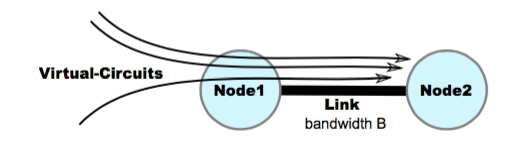
\includegraphics[width=100mm,scale=1]{imagensGuia/ex1.png}
 \label{fig:ex1}
\end{figure}

\subsection{Exercício 1 e 2}

Nestes primeiros exercícios era pedido que se obtivesse os valores de probabilidade de bloqueio e de carga média do link, tanto de forma simulada como teórica, para vários valores de $\lambda$ (média de pedidos de chamadas por minuto), 1/$\mu$ (média da duração de cada chamada, em minutos), onde cada circuito virtual (VC), requer uma largura de banda de 2 Mbits/sec e o link pode tomar vários valores de largura de banda.


Foram obtidos os seguintes resultados para cada valor de largura de banda do link:

\begin{figure}[!htb]
\center
 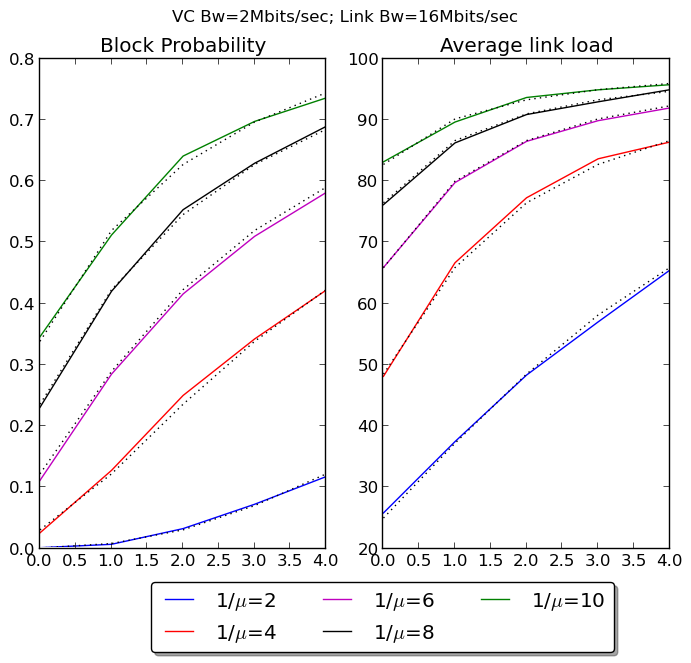
\includegraphics[width=90mm,scale=1]{imagensGuia/graph1ex1.png}
 \label{fig:graph1ex1}
 \caption{Probabilidade de bloqueio e carga média do link com 16 Mbits/sec}
\end{figure}

\newpage
\begin{figure}[!htb]
\center
 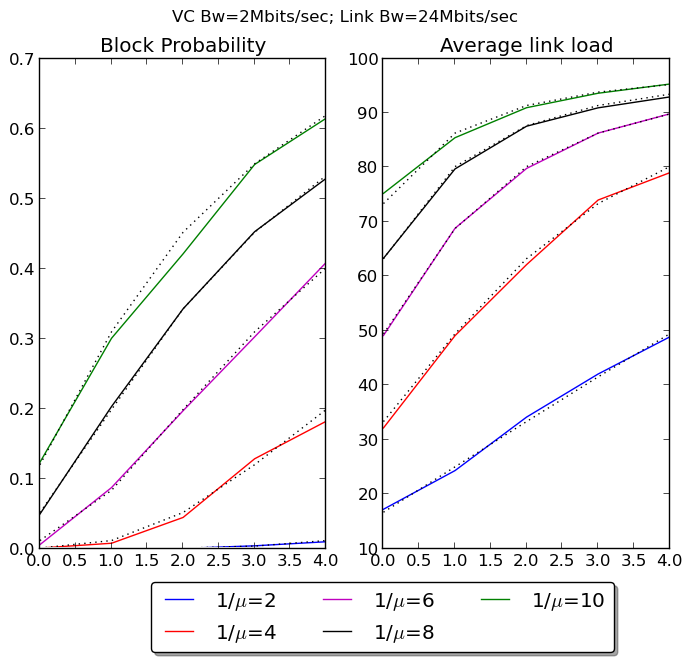
\includegraphics[width=90mm,scale=1]{imagensGuia/graph2ex1.png}
 \label{fig:graph2ex1}
 \caption{Probabilidade de bloqueio e carga média do link com 24 Mbits/sec}
\end{figure}

\begin{figure}[!htb]
\center
 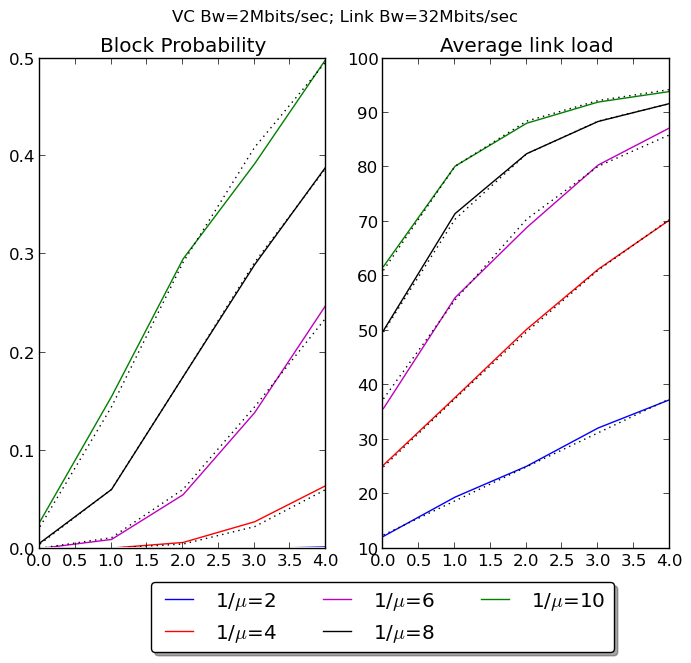
\includegraphics[width=90mm,scale=1]{imagensGuia/graph3ex1.png}
 \label{fig:graph3ex1}
 \caption{Probabilidade de bloqueio e carga média do link com 32 Mbits/sec} 
\end{figure}

Nos três casos, é possível observar-se o valor simulado (linha contínua) e o valor teórico (linha picotada), para os vários tempos médios de duração de uma chamada.

Através da figura 1, onde a largura de banda do link é de 16 Mbits/seg é possível ver que a probabilidade de bloqueio é muito maior, comparando com a figura 3, onde a largura de banda é o dobro, 32 Mbits/sec. Como existe mais largura de banda no link, para um mesmo número de pedidos de chamadas, estas bloqueiam em menos quantidade, pois é possível processar um maior número de pedidos. 

Em todos os gráficos, é possível observar-se que à medida que a taxa de chamadas vai aumentando, a probabilidade de bloqueio e a ocupação média do link também vão aumentar, pois são mais pedidos para processar.

Relativamente à duração das chamadas, quando esta aumenta, a probabilidade de bloqueio e a ocupação média do link também vão aumentar, pois as chamadas ocuparão por mais tempo o link, com a mesma taxa de pedidos.

\newpage
\subsection{Exercício 3}

Neste terceiro exercício, as chamadas passaram a ser de dois tipos, um standard e um special. As chamadas standard requerem uma largura de banda de 2 Mbits/sec e as special requerem uma largura de banda de 4 Mbits/sec. Neste caso, os nós possuem ainda uma quantidade de Mbit/s reservados para os pedidos especiais. Foram obtidos os resultados da simulação para vários valores de $\lambda$ standard e special, 1/$\mu$, largura de banda do link e largura de banda reservada.

Obtiveram-se os seguintes resultados, através da execução de 3 amostras:

\begin{figure}[!htb]
  \centering
  \begin{minipage}[b]{0.4\textwidth}
    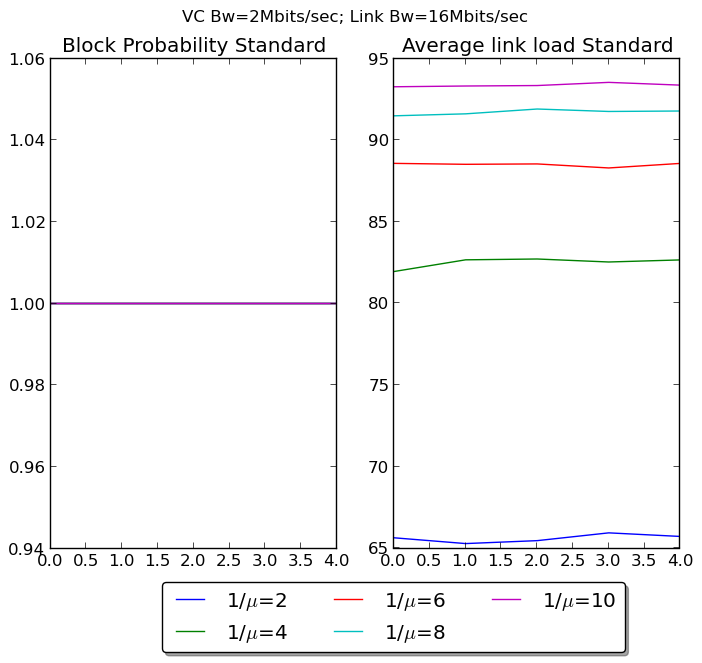
\includegraphics[width=\textwidth]{imagensGuia/graphstandard1ex3.png}
  \end{minipage}
  \hfill
  \begin{minipage}[b]{0.4\textwidth}
    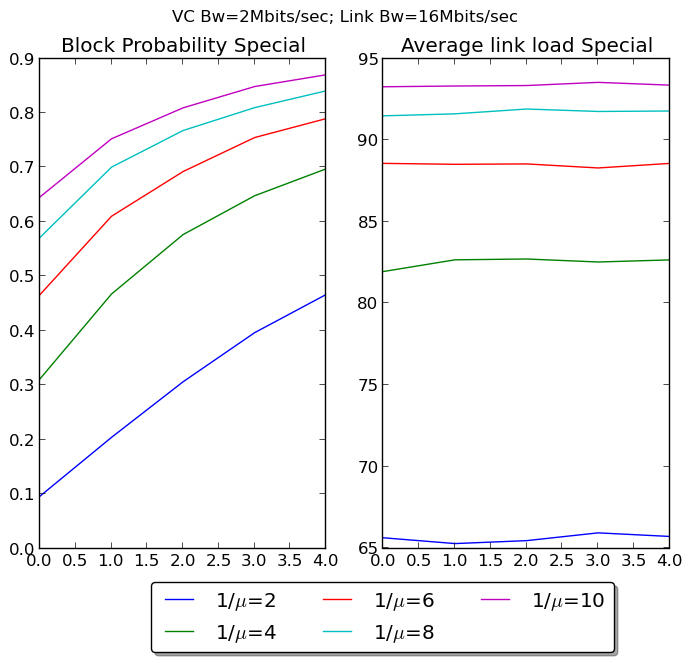
\includegraphics[width=\textwidth]{imagensGuia/graphspecial2ex3}
  \end{minipage}
  \caption{Probabilidade de bloqueio dos pedidos standard e special e ocupação média do link com 16 Mbits/sec}
\end{figure}

\begin{figure}[!htb]
  \centering
  \begin{minipage}[b]{0.4\textwidth}
    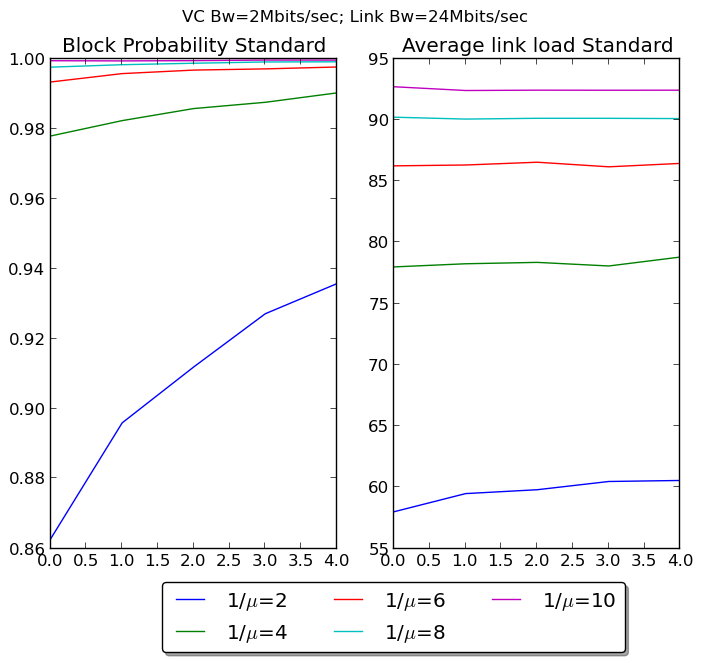
\includegraphics[width=\textwidth]{imagensGuia/graphstandard3ex3.png}
  \end{minipage}
  \hfill
  \begin{minipage}[b]{0.4\textwidth}
    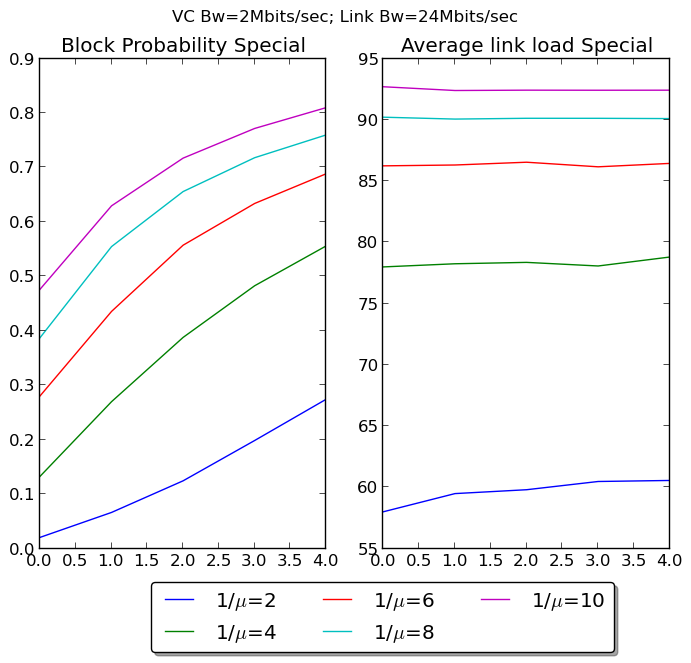
\includegraphics[width=\textwidth]{imagensGuia/graphspecial4ex3}
  \end{minipage}
  \caption{Probabilidade de bloqueio dos pedidos standard e special e ocupação média do link com 24 Mbits/sec}
\end{figure}
\newpage
\begin{figure}[!htb]
  \centering
  \begin{minipage}[b]{0.4\textwidth}
    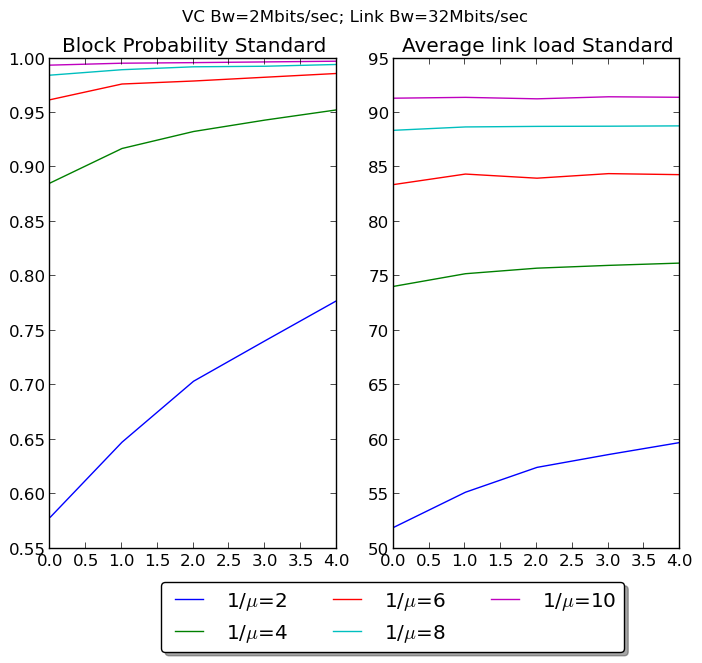
\includegraphics[width=\textwidth]{imagensGuia/graphstandard5ex3.png}
  \end{minipage}
  \hfill
  \begin{minipage}[b]{0.4\textwidth}
    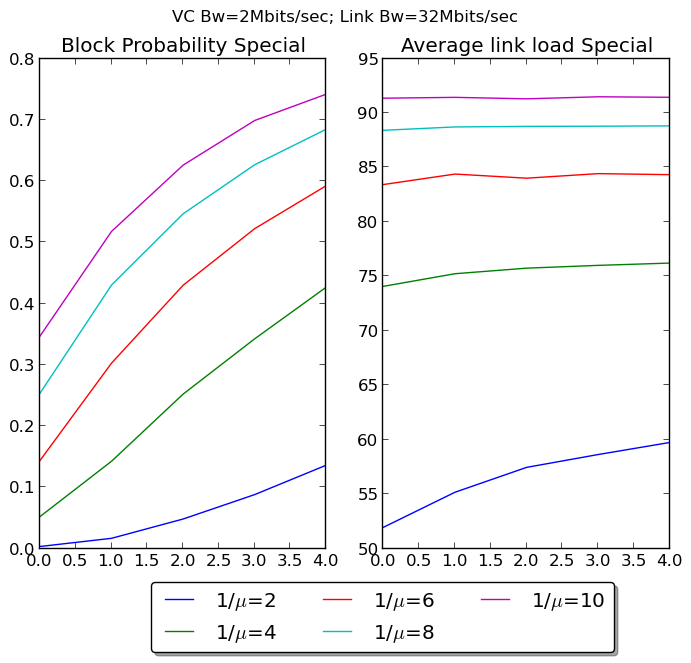
\includegraphics[width=\textwidth]{imagensGuia/graphspecial6ex3}
  \end{minipage}
  \caption{Probabilidade de bloqueio dos pedidos standard e special e ocupação média do link com 32 Mbits/sec}
\end{figure}

Observando os gráficos acima, é possível observar-se que quanto maior for a capacidade do link, os pedidos standard, começam a bloquear menos vezes. É possível verificar que quanto maior o valor de largura de banda reservada, melhores serão os pedidos special, e pior os standard. 

Na figura 4, o link possuí uma largura de banda de 16 Mbits/sec, e a largura de banda reservada, sendo 16 Mbits/sec, faz com que os pedidos standard bloqueiem 100\% das vezes, pois toda a largura de banda existente está disponível apenas para os pedidos special.

Nas figuras 5 e 6, o valor da largura de banda do link vai aumentado. Com isto, a probabilidade de bloqueio dos pedidos standard vai diminuindo. A maior diminuição verifica-se quando a duração dos pedidos é a mais curta, linha azul, isto porque, tal como se verificou no primeiro exercício quanto mais baixa for a duração do pedido, menor será a probabilidade de bloqueio.

Com o aumento da largura de banda do link, os pedidos especiais também terão menor probabilidade de bloqueio, tal como se verificou no exercício 1.

Para este exercício foram criados dois geradores de pedidos, um para pedidos standard, e outro para pedidos special.

\newpage
\section{Packet Switched Network - Single-queue simulation}
\subsection{Exercício 4 e 5}

\begin{figure}[!htb]
\center
 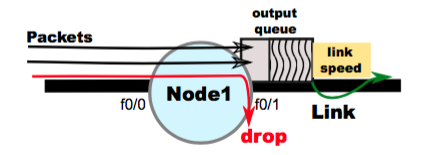
\includegraphics[width=100mm,scale=1]{imagensGuia/ex4.png}
 \label{fig:ex4}
\end{figure}

Nestes exercícios, a ideia passa pela simulação de routers. Tal como mostra a figura acima, agora existe uma fila de espera à entrada do node que depende da velocidade de comutação do router, e uma de saída, que vai depender do processamento do link.
Caso chegue um pacote e a fila estiver cheia, este é perdido, caso contrário, ficará à espera havendo atraso.
À saída do router o tempo de saída do mesmo, vai depender do tamanho do pacote.

Neste exemplo, o Node 1 é um router, com uma velocidade de processamento muito elevada, conectado a um link de 2 Mbits/sec. Para a fila de espera de entrada do Node, considerou-se um tamanho infinito. Para a fila de espera de saída, são utilizados vários valores (64, 96, 128, 10000), para vários testes. 

O tamanho dos pacotes, segue uma distribuição exponencial com probabilidade de 50\% para 64 bytes e 50\% para 1500 bytes.

O tempo entre o envio de pacotes, segue também uma distribuição exponencial com média 1/$\lambda$, onde o valor de $\lambda$ pode tomar diferentes valores (150, 300, 450).

Nestes exercícios, para além do cálculo da percentagem de pacotes perdidos, atraso médio dos pacotes e largura de banda transmitida, era pedido também que se calculasse o atraso através das seguintes fórmulas, para comparar com o valor simulado:

\begin{itemize}
\item M/M/1, uma fórmula mais viável quando os pacotes são praticamente todos do mesmo tamanho, dando apenas bons resultados, quando existem poucos pacotes.
\item M/D/1, apenas depende do número de pacotes e não do tamanho dos mesmo. Funciona apenas bem à entrada, contudo à saída não, pois nada é determinístico à saída.
\item M/G/1 (geral), as fórmulas neste caso, dependem da média e da variância do serviço. Funciona melhor quando as coisas já não são tão exponenciais.
\item M/M/1/K, quando a fila de espera é limitada, utiliza-se estas fórmulas, para obter a probabilidade de perda do pacote.
\end{itemize}

Na tabela seguinte, é possível verificar-se os valores que se obtiveram no final dos testes. Nestes testes o tempo de simulação foi de 30 e para as filas de espera de 10000, foi de 500, de forma a conseguir-se encher estas filas e obter-se valores pretendidos. Foram simuladas 3 amostras, obtendo-se os seguintes valores:

\begin{table}[!htb]
\centering
\resizebox{\textwidth}{!}{\begin{tabular}{llllllllll}
\rowcolor[HTML]{FFCC67} 
lambda & queueSize & Loss probability & Average delay & Transmitted bandwidth & M/M/1    & M/D/1    & M/G/1   & M/M/1/K  & M/M/1/K\% \\
150    & 64        & 0.02252          & 0.00545       & 114028.8              & 0.00589  & 0.00451  & 0.00385 & 0.00589  & 0         \\
150    & 96        & 0                & 0.00553       & 116283.73333          & 0.00589  & 0.00451  & 0.00385 & 0.00589  & 0         \\
150    & 128       & 0.03356          & 0.00567       & 115715.73333          & 0.00589  & 0.00451  & 0.00385 & 0.00589  & 0         \\
150    & 10000     & 0.00333          & 0.00563       & 117320.584            & 0.00589  & 0.00451  & 0.00385 & 0.00589  & 0         \\
300    & 64        & 0.05506          & 0.04444       & 236680                & 0.05078  & 0.02695  & 0.00329 & 0.0473   & 0.10701   \\
300    & 96        & 0.23815          & 0.04378       & 232942.2              & 0.05078  & 0.02695  & 0.00329 & 0.05011  & 0.0138    \\
300    & 128       & 0.06061          & 0.04398       & 237527.73333          & 0.05078  & 0.02695  & 0.00329 & 0.05066  & 0.0018    \\
300    & 10000     & 0.01529          & 0.04662       & 234915.284            & 0.05078  & 0.02695  & 0.00329 & 0.05078  & 0         \\
450    & 64        & 29.26271         & 0.19105       & 249873.8              & -0.00767 & -0.00227 & 0.00147 & 0.19252  & 28.95709  \\
450    & 96        & 28.7556          & 0.28939       & 249918.8              & -0.00767 & -0.00227 & 0.00147 & 0.29261  & 28.95709  \\
450    & 128       & 29.42856         & 0.38974       & 249927.53333          & -0.00767 & -0.00227 & 0.00147 & 0.39271  & 28.95709  \\
450    & 10000     & 29.0788          & 27.86529      & 249995.904            & -0.00767 & -0.00227 & 0.00147 & 31.27233 & 28.95709 
\end{tabular}}
\caption[]{Valores teóricos e simulados do atraso e da probabilidade de perda de pacotes \footnotemark}
\end{table}

\footnotetext{Todos os valores das tabelas são uma média de várias amostras}

Este primeiro caso, os pacotes são perdidos à saída do router, pelo que a fórmulas M/M/1 e M/M/1/K, são as que se aproximam mais dos valores reais. Pode-se verificar que a fórmula de M/M/1 para poucos pacotes, tal como descrito acima, funciona melhor. Neste caso, para um valor $\lambda$ de 150 ou 300, esta fórmula funciona bem, mas para um valor mais elevado, como 450, esta fórmula falha. Esta falha é observada, pelo valor negativo que se obtém. A fórmula M/M/1/K, funciona sempre para qualquer tipo de valores.

Sendo os pacotes perdidos à saída, a fórmula M/D/1, falha para valores elevados de $\lambda$, e também não é muito precisa para os outros valores, tal como descrito acima, esta fórmula funciona melhor à entrada do router.

A fórmula M/G/1, não falha, contudo os valores fogem muito do pretendido, pois são valores exponenciais.

\newpage
\subsection{Exercício 6 e 7}

\begin{figure}[!htb]
\center
 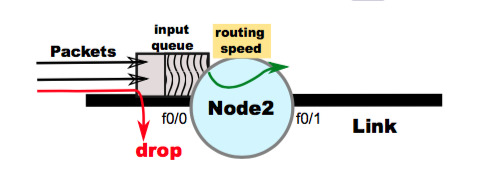
\includegraphics[width=100mm,scale=1]{imagensGuia/ex6.png}
 \label{fig:ex6}
\end{figure}

Nestes exercícios, a perda de pacotes agora ocorre na entrada do router. Para isso, assumiu-se uma fila de espera finita à entrada que pode tomar vários valores (64, 96, 128, 10000) e uma fila infinita à saída. Neste caso a velocidade do link não terá qualquer influência, pois este é muito rápido, 10 Gbits/sec. No entanto, o router tem uma velocidade de processamento lenta, de 350 pacotes/sec.

O tamanho dos pacotes e o tempo entre dois pacotes são os mesmos do exercício anterior.

Foi então pedido que se efetuassem os mesmos cálculos e os mesmos testes para comparação dos valores simulados com os valores teóricos. Utilizou-se os mesmos tempos de simulação do exercício anterior e o mesmo número de simulações. A tabela seguinte mostra os resultados obtidos: 

\begin{table}[!htb]
\centering
\resizebox{\textwidth}{!}{\begin{tabular}{llllllllll}
\rowcolor[HTML]{FFCC67} 
lambda & queueSize & Loss probability & Average delay & Transmitted bandwidth & M/M/1 & M/D/1    & M/G/1   & M/M/1/K  & M/M/1/K\% \\
150    & 64        & 0                & 0.0039        & 117129.46667          & 0.005 & 0.00393  & 0.00321 & 0.005    & 0         \\
150    & 96        & 0                & 0.00391       & 115831.4              & 0.005 & 0.00393  & 0.00321 & 0.005    & 0         \\
150    & 128       & 0.01067          & 0.00399       & 119278.93333          & 0.005 & 0.00393  & 0.00321 & 0.005    & 0         \\
150    & 10000     & 0.00134          & 0.00394       & 117086.284            & 0.005 & 0.00393  & 0.00321 & 0.005    & 0         \\
300    & 64        & 0.12112          & 0.01209       & 233961.66667          & 0.02  & 0.01143  & 0.00303 & 0.01999  & 0.00074   \\
300    & 96        & 0.06705          & 0.01095       & 232275.6              & 0.02  & 0.01143  & 0.00303 & 0.02     & 0.00001   \\
300    & 128       & 0.0111           & 0.01179       & 233451.53333          & 0.02  & 0.01143  & 0.00303 & 0.02     & 0         \\
300    & 10000     & 0.00266          & 0.01134       & 234246.852            & 0.02  & 0.01143  & 0.00303 & 0.02     & 0         \\
450    & 64        & 22.56702         & 0.178         & 271494.93333          & -0.01 & -0.00357 & 0.00233 & 0.17286  & 22.22222  \\
450    & 96        & 22.79043         & 0.26636       & 272059.73333          & -0.01 & -0.00357 & 0.00233 & 0.26429  & 22.22222  \\
450    & 128       & 22.31655         & 0.35297       & 272260.8              & -0.01 & -0.00357 & 0.00233 & 0.35571  & 22.22222  \\
450    & 10000     & 22.29851         & 24.90259      & 274311.352            & -0.01 & -0.00357 & 0.00233 & 28.56143 & 22.22222 
\end{tabular}}
\caption[]{Valores teóricos e simulados do atraso e da probabilidade de perda de pacotes \footnotemark}
\end{table}

\footnotetext{Todos os valores das tabelas são uma média de várias amostras}

Olhando para a tabela, verifica-se que a fórmula de M/M/1, neste caso, que a fila de espera se encontra à entrada do router, não funciona como no exemplo anterior, fugindo bastante dos valores desejados.

Como também já foi referido, a fórmula M/D/1 funciona melhor à entrada do router, como neste caso. Com isto, é possível verificar que os valores são bastante próximos  dos desejados para valores de $\lambda$ mais pequenos, tal como a fórmula M/M/1, no exemplo anterior.

A fórmula de M/G/1, funciona bem para um valor de $\lambda$ mais pequeno como é o caso de 150, mas para os outros valores, 300 e 450, começa a ficar longe dos resultados desejados.

Neste caso, é possível verificar que mais uma vez, a fórmula de M/M/1/K é a mais eficiente, tanto a nível de percentagem de pacotes perdidos, como de atraso. Para qualquer valor de $\lambda$, esta fórmula aproxima-se sempre do valor pretendido.

\subsection{Exercício 8}

\subsubsection{Geração dos pacotes}
Para gerar os pacotes, usou-se a amostra gerada no guia anterior para os ON/OFF. A amostra que foi criada, foi criada representando número de bytes.

Sendo assim, iterou-se sobre a lista que representa a amostra e cada entrada da lista corresponde ao número de bytes por segundo enviados. Como pretendemos que o número seja em número de pacotes e não em número de bytes, dividiu-se, cada entrada da lista ou por 64 ou por 1500 com probabilidades iguais, 50-50.

Depois, para saber o instante de saída de cada pacote, dividiu-se um segundo pelo número de pacotes enviados.

Quando o número de pacotes enviados é igual a zero, e existe um intervalo de pacotes enviados igual a zero, soma-se ao anterior.

O lambda corresponde à media de pacotes recebidos por segundo.

O código python com o raciocínio descrito está no ficheiro: extra8\_generate.py.

\subsubsection{Modificação do pkt\_Sender}

Adicionou-se ao pkt\_sender um argumento: "list\_pkts" que corresponde à lista com o número de pacotes e os seus respetivos intervalos.

\begin{lstlisting}[language=python]
def __init__(self, env, id, dst, list_pkts):
\end{lstlisting}

Depois é efetuada uma iteração sobre a lista e para cada entrada da lista, se o "number\_of\_packets" for igual a 0, não será enviado nenhum pacote:

\begin{lstlisting}[language=python]
time = pkt_l["time"]
simtime += time

yield self.env.timeout(time)
\end{lstlisting}

Caso seja diferente,  iremos enviar um pacote, com 64 ou 1500 bytes com probabilidade de 50-50.

O código python com o raciocínio descrito está no ficheiro: extra8.py.

\subsubsection{Análise dos resultados}

Os resultados obtidos para ambos os Nodes simulados foram os seguintes:

\begin{table}[!htb]
\centering
\resizebox{\textwidth}{!}{\begin{tabular}{llllllllll}
\rowcolor[HTML]{FFCC67} 
lambda & queueSize & Loss probability & Average delay & Transmitted bandwidth & M/M/1   & M/D/1   & M/G/1   & M/M/1/K & M/M/1/K\% \\
275    & 64        & 85.82314         & 0.14296       & 30580.01333           & 0.02237 & 0.01275 & 0.00347 & 0.02236 & 0.00091   \\
275    & 96        & 84.90369         & 0.20026       & 16297.18667           & 0.02237 & 0.01275 & 0.00347 & 0.02237 & 0.00001   \\
275    & 128       & 84.05209         & 0.25237       & 17164.36667           & 0.02237 & 0.01275 & 0.00347 & 0.02237 & 0         \\
275    & 10000     & 13.61478         & 14.94243      & 92469.32              & 0.02237 & 0.01275 & 0.00347 & 0.02237 & 0        
\end{tabular}}
\caption{Valores teóricos e simulados do atraso e da probabilidade de perda de pacotes no Node 1}
\end{table}

\begin{table}[!htb]
\centering
\resizebox{\textwidth}{!}{\begin{tabular}{llllllllll}
\rowcolor[HTML]{FFCC67} 
lambda & queueSize & Loss probability & Average delay & Transmitted bandwidth & M/M/1   & M/D/1  & M/G/1  & M/M/1/K & M/M/1/K\% \\
275    & 64        & 84.90248         & 0.12804       & 32245.16              & 0.01333 & 0.0081 & 0.0031 & 0.01333 & 0         \\
275    & 96        & 84.03998         & 0.18          & 34316.50667           & 0.01333 & 0.0081 & 0.0031 & 0.01333 & 0         \\
275    & 128       & 83.26469         & 0.22815       & 36109.22667           & 0.01333 & 0.0081 & 0.0031 & 0.01333 & 0         \\
275    & 10000     & 12.24712         & 13.52609      & 188444                & 0.01333 & 0.0081 & 0.0031 & 0.01333 & 0        
\end{tabular}}
\caption{Valores teóricos e simulados do atraso e da probabilidade de perda de pacotes no Node 2}
\end{table}

Neste exercício, deixou-se de ter um conjunto de $\lambda$ e passou-se a ter um único valor de $\lambda$, neste caso 275, número total de pacotes a dividir pelo tempo de simulação.

Através das tabelas acima, verifica-se que os valores teóricos são muito diferentes dos valores reais, pois estes valores estão longe de ser uma distribuição exponencial, pelo que se pode concluir que as fórmulas utilizadas, falham para tráfego realista. 

\newpage
\section{Packet Switched Network - Multi-queue simulation}

\subsection{Exercício 9 e 10}

\begin{figure}[!htb]
\center
 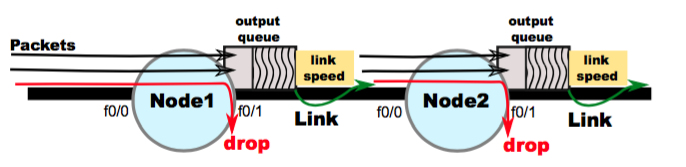
\includegraphics[width=100mm,scale=1]{imagensGuia/ex9.png}
 \label{fig:ex9}
\end{figure}

Assumindo agora que a rede possui dois routers (Node 1 e Node 2), com uma velocidade de processamento bastante elevada e ligados a links de 2 Mbits/sec. Ambos possuem na sua saída filas de espera finitas que podem tomar diferentes valores (64, 96, 128, 10000) e na sua entrada assume-se que as filas de espera são infinitas. Este caso é mais adequado a um cenário de operador.

Utilizando os mesmos valores de $\lambda$ utilizados anteriormente (150, 300, 450) foi pedido que se calculasse utilizando a aproximação de Kleinrock, o atraso médio de um pacote e a sua probabilidade de perda.

O atraso total do sistema é calculado através da soma de todos os atrasos em todas as filas de espera.

Em todas as filas de espera é necessário calcular o $\lambda$. Existe ainda $\gamma$, que consiste em tudo o que está a entrar na rede, pelo que se soma todos os atrasos com a seguinte fórmula:

\[W = \frac{1}{\gamma}\times\left[\frac{\lambda_{1}}{\left(\mu-\lambda_{1}\right)}+\frac{\lambda_{2}}{\left(\mu-\lambda_{2}\right)}\right]\]

Sendo que assumindo que  $\lambda_{1}$ = $\lambda_{2}$ = $\lambda$ = $\gamma$, temos que:

\[W = \frac{2}{\left(\mu-\lambda\right)}\]

\newpage
Utilizando esta fórmula, os resultados simulados e teóricos obtidos, num conjunto de 3 simulações, com um tempo de simulação de 500 para a fila de espera de tamanho 10000 e 30 para as restantes filas de espera, foram os apresentados na tabela seguinte:

\begin{table}[!htb]
\centering
\resizebox{\textwidth}{!}{\begin{tabular}{llllll}
\rowcolor[HTML]{FFCC67} 
lambda & queueSize & Loss Probability & Average Delay & Transmitted bandwidth & Wk       \\
150    & 64        & 0.0111           & 0.01026       & 115840.66667          & 0.01179  \\
150    & 96        & 0.09048          & 0.01021       & 114507.2              & 0.01179  \\
150    & 128       & 0.06658          & 0.01053       & 120261.73333          & 0.01179  \\
150    & 10000     & 0.002            & 0.01047       & 117425.848            & 0.01179  \\
300    & 64        & 0.29014          & 0.04365       & 230875.46667          & 0.10156  \\
300    & 96        & 0.22997          & 0.04345       & 230808.86667          & 0.10156  \\
300    & 128       & 0.36015          & 0.06956       & 235875.2              & 0.10156  \\
300    & 10000     & 0.01232          & 0.05448       & 234914.136            & 0.10156  \\
450    & 64        & 29.88578         & 0.20224       & 249782.33333          & -0.01535 \\
450    & 96        & 29.2007          & 0.29619       & 249801.13333          & -0.01535 \\
450    & 128       & 28.68136         & 0.38949       & 249821.06667          & -0.01535 \\
450    & 10000     & 29.18195         & 27.96119      & 249992.316            & -0.01535
\end{tabular}}
\caption[]{Valores teóricos e simulados do atraso e da probabilidade de perda de pacotes utilizando a aproximação de Kleinrock \footnotemark}
\end{table}

\footnotetext{Todos os valores das tabelas são uma média de várias amostras}

Através da tabela acima, observa-se que a aproximação de Kleinrock, para calcular o atraso do sistema, funciona bem para valores baixos de $\lambda$, como 150, sendo que quando este valor aumenta, começa a fugir do resultado pretendido, até que numa quantidade de 450 pacotes/s, deixa mesmo de ser uma opção viável, pois a fórmula falha. Uma solução para prevenir esta falha, seria aumentar a largura de banda dos links, de forma a que a aproximação não desse valores negativos.
\newpage
\subsection{Exercício 11}
\begin{figure}[!htb]
\center
 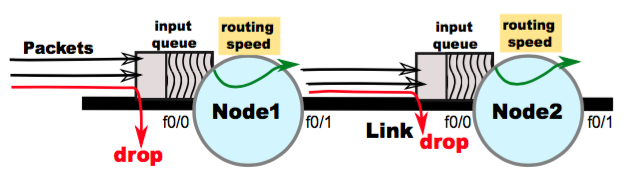
\includegraphics[width=100mm,scale=1]{imagensGuia/ex11.png}
 \label{fig:ex11}
\end{figure}

Neste exercício, o objetivo era a comparação dos valores simulados e teóricos do atraso, utilizando uma aproximação de Kleinrock.

Nesta situação, e como se pode ver na imagem acima, existem dois nodes lentos, só interessando assim, as filas de espera de entrada, pois o link é bastante rápido, com 10 Gbits/s de largura de banda. A velocidade de processamento dos nodes é de 350 pacotes. Este cenário é o mais frequente em empresas.

Com isto obtiveram-se os seguintes valores, utilizando os mesmos critérios (tempo de simulação e simulações efetuadas) das simulações anteriores:

\begin{table}[!htb]
\centering
\resizebox{\textwidth}{!}{\begin{tabular}{llllll}
\rowcolor[HTML]{FFCC67} 
lambda & queueSize & Loss Probability & Average Delay & Transmitted bandwidth & Wk    \\
150    & 64        & 0.01101          & 0.00673       & 117924.53333          & 0.01  \\
150    & 96        & 0.02255          & 0.00675       & 114169.66667          & 0.01  \\
150    & 128       & 0                & 0.00674       & 115667.4              & 0.01  \\
150    & 10000     & 0.00133          & 0.00678       & 117166.072            & 0.01  \\
300    & 64        & 0.04449          & 0.01408       & 232950.93333          & 0.04  \\
300    & 96        & 0.09951          & 0.01362       & 237435.86667          & 0.04  \\
300    & 128       & 0.09956          & 0.01463       & 236368                & 0.04  \\
300    & 10000     & 0.00468          & 0.014         & 233576.692            & 0.04  \\
450    & 64        & 22.3342          & 0.18101       & 272711.26667          & -0.02 \\
450    & 96        & 21.87301         & 0.26995       & 273241                & -0.02 \\
450    & 128       & 21.2317          & 0.35386       & 269315.93333          & -0.02 \\
450    & 10000     & 22.3274          & 24.90107      & 273435.2              & -0.02
\end{tabular}}
\caption[]{Valores teóricos e simulados do atraso e da probabilidade de perda de pacotes utilizando a aproximação de Kleinrock \footnotemark}
\end{table}

\footnotetext{Todos os valores das tabelas são uma média de várias amostras}

Como agora o valor de $\mu$ é igual ao valor do routing speed, 350, então para todas as filas de espera, o valor de Wk é igual para cada $\lambda$. Quando o valor de $\lambda$ é mais pequeno, o atraso obtido teoricamente aproxima-se do valor simulado. Tal como nos caso anterior quando maior o valor de $\lambda$, mais probabilidade tem  a fórmula de falhar.

\newpage
\subsection{Exercício 12}
\begin{figure}[!htb]
\center
 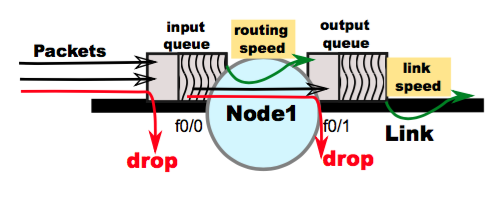
\includegraphics[width=100mm,scale=1]{imagensGuia/ex12.png}
 \label{fig:ex12}
\end{figure}

Neste exercício, voltou-se a utilizar apenas um router (Node 1), onde a sua velocidade de processamento é de 300 pacotes/s e possui duas filas de espera, entrada e saída, finitas, ambas com a mesma capacidade (64, 96, 128, 10000). Este nó está ainda conectado a um link com velocidade de 2 Mbits/sec.

Foi pedido que através da aproximação de Kleinrock, se comparassem os valores de atraso simulados com os valores teóricos, oriundos desta aproximação. Obtiveram-se os seguintes resultados, utilizando os mesmos tempos de simulação e o mesmo número de simulações efetuadas nos exercícios anteriores:

\begin{table}[!htb]
\centering
\resizebox{\textwidth}{!}{\begin{tabular}{llllll}
\rowcolor[HTML]{FFCC67} 
lambda & queueSize & Loss Probability & Average Delay & Transmitted bandwidth & Wk       \\
150    & 64        & 0.01118          & 0.00986       & 117543.4              & 0.01179  \\
150    & 96        & 0.03317          & 0.0099        & 117739.33333          & 0.01179  \\
150    & 128       & 0.01115          & 0.00984       & 116991                & 0.01179  \\
150    & 10000     & 0.00067          & 0.00987       & 117620.648            & 0.01179  \\
300    & 64        & 1.37433          & 0.13872       & 233642.73333          & 0.10156  \\
300    & 96        & 0.41959          & 0.11477       & 230754.73333          & 0.10156  \\
300    & 128       & 0.78062          & 0.16925       & 230433.4              & 0.10156  \\
300    & 10000     & 0.12461          & 0.74235       & 234200.228            & 0.10156  \\
450    & 64        & 33.16216         & 0.23206       & 234946.2              & -0.01535 \\
450    & 96        & 33.29091         & 0.33406       & 233296.93333          & -0.01535 \\
450    & 128       & 33.08208         & 0.43899       & 234862.66667          & -0.01535 \\
450    & 10000     & 33.52031         & 29.98766      & 234454.452            & -0.01535
\end{tabular}}
\caption[]{Valores teóricos e simulados do atraso e da probabilidade de perda de pacotes utilizando a aproximação de Kleinrock \footnotemark}
\end{table}

\footnotetext{Todos os valores das tabelas são uma média de várias amostras}

Como o cálculo deste atraso é feito através da fórmula apresentada acima, os valores teóricos vão ser iguais, pelo que os valores de $\lambda$ e $\mu$ são iguais. Contudo nesta situação, para além de se aproximar dos valores simulados com um $\lambda$ de 150, também se aproxima ligeiramente dos valores simulados com um $\lambda$ de 300. Contudo, continua a falhar no caso dos 450 pacotes/s, isto porque agora a capacidade de processamento do router interessa, e é de 300 pacotes/s, pelo que valores acima disso, como o caso de 450, já faz com que haja uma perda de pacotes maior.

\newpage
\section{Multi-queue simulation with routing}

\subsection{Exercício 13}
\begin{figure}[!htb]
\center
 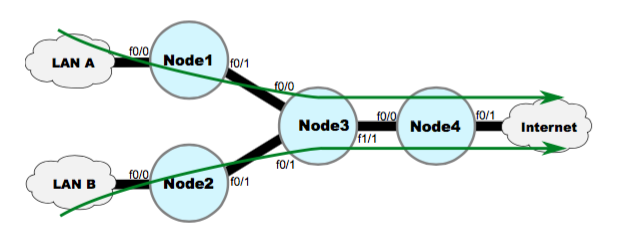
\includegraphics[width=100mm,scale=1]{imagensGuia/ex13.png}
 \label{fig:ex13}
\end{figure}

Neste últimos exercícios era pretendido que se simulasse o transporte de pacotes de duas redes diferentes para a Internet. Como se pode ver na imagem acima, vão existir 6 filas de espera, antes e depois de cada router, pelo que será necessário calcular a soma de todos os atrasos.
6 filas de espera, e é necessário somar os atrasos

Neste caso, todos os links terão uma largura de banda de banda de 10 Mbits/sec, e a velocidade de processamento do router pode tomar vários valores (500, 750, 1000). Tanto a LAN A, como a LAN B, podem tomar vários valores de $\lambda$, 150, 300, 450, 600, no entanto para este guia, utilizaram-se os valores de 150 e 600. O tamanho das filas de espera pode também tomar vários valores, 64, 96, 128, 192, 256, sendo que apenas se utilizou 64 e 256.

Os resultados obtidos foram os seguintes, com um tempo de simulação de 200 e efetuaram-se 3 simulações:

\begin{table}[!htb]
\centering
\resizebox{\textwidth}{!}{\begin{tabular}{lllllllllll}
\rowcolor[HTML]{FFCC67} 
lambdaAI & lambdaBI & queueSize & R    & B        & Loss Probability nodes & Loss Probability links & Loss Probability & Average Delay & Transmitted bandwidth & Wk       \\
150      & 150      & 64        & 500  & 10000000 & 0                      & 0                      & 0                & 0.00982       & 233827.82             & 0.01509  \\
150      & 150      & 64        & 750  & 10000000 & 0                      & 0                      & 0                & 0.00663       & 233577.3              & 0.00834  \\
150      & 150      & 64        & 1000 & 10000000 & 0                      & 0                      & 0                & 0.0054        & 233979.32             & 0.00626  \\
150      & 150      & 256       & 500  & 10000000 & 0                      & 0                      & 0                & 0.00977       & 232979.78             & 0.01509  \\
150      & 150      & 256       & 750  & 10000000 & 0                      & 0                      & 0                & 0.00662       & 232961.94             & 0.00834  \\
150      & 150      & 256       & 1000 & 10000000 & 0                      & 0                      & 0                & 0.0054        & 233344.6              & 0.00626  \\
150      & 600      & 64        & 500  & 10000000 & 33.35175               & 0                      & 33.35175         & 0.24613       & 361545.4              & -0.01213 \\
150      & 600      & 64        & 750  & 10000000 & 0.80478                & 0                      & 0.80478          & 0.05317       & 583628.86             & 0.00896  \\
150      & 600      & 64        & 1000 & 10000000 & 0                      & 0                      & 0                & 0.00745       & 587890.16             & 0.01353  \\
150      & 600      & 256       & 500  & 10000000 & 32.85452               & 0                      & 32.85452         & 0.97383       & 360799.32             & -0.01213 \\
150      & 600      & 256       & 750  & 10000000 & 0.30115                & 0                      & 0.30115          & 0.19829       & 585577.56             & 0.00896  \\
150      & 600      & 256       & 1000 & 10000000 & 0                      & 0                      & 0                & 0.00746       & 587321.62             & 0.01353  \\
600      & 150      & 64        & 500  & 10000000 & 33.51197               & 0                      & 33.51197         & 0.23854       & 451030.38             & -0.01213 \\
600      & 150      & 64        & 750  & 10000000 & 0.56011                & 0                      & 0.56011          & 0.0491        & 582928.5              & 0.00896  \\
600      & 150      & 64        & 1000 & 10000000 & 0                      & 0                      & 0                & 0.00745       & 586636.96             & 0.01353  \\
600      & 150      & 256       & 500  & 10000000 & 32.92378               & 0                      & 32.92378         & 0.92027       & 456723.48             & -0.01213 \\
600      & 150      & 256       & 750  & 10000000 & 0.20351                & 0                      & 0.20351          & 0.20534       & 584107.84             & 0.00896  \\
600      & 150      & 256       & 1000 & 10000000 & 0                      & 0                      & 0                & 0.00746       & 587001.24             & 0.01353  \\
600      & 600      & 64        & 500  & 10000000 & 58.27027               & 0                      & 58.27027         & 0.25779       & 300473.28             & -0.00684 \\
600      & 600      & 64        & 750  & 10000000 & 37.59938               & 0                      & 37.59938         & 0.09361       & 679479.08             & 0.00824  \\
600      & 600      & 64        & 1000 & 10000000 & 16.5951                & 0                      & 16.5951          & 0.07278       & 844541.46             & -0.00148 \\
600      & 600      & 256       & 500  & 10000000 & 58.01832               & 0                      & 58.01832         & 1.02029       & 390560.74             & -0.00684 \\
600      & 600      & 256       & 750  & 10000000 & 37.47508               & 0                      & 37.47508         & 0.34891       & 679716.34             & 0.00824  \\
600      & 600      & 256       & 1000 & 10000000 & 16.69364               & 0                      & 16.69364         & 0.26385       & 844699.74             & -0.00148
\end{tabular}}
\caption[]{Valores teóricos e simulados do atraso e da probabilidade de perda de pacotes utilizando a aproximação de Kleinrock \footnotemark}
\end{table}

\footnotetext{Todos os valores das tabelas são uma média de várias amostras}

Através da tabela apresentada acima, é possível observar-se que quando ambas as LAN's enviam pacotes com uma taxa de 150 pacotes por segundo, não existe perda de pacotes, qualquer que seja o valor de R, routing speed.

Quando, por exemplo uma das LAN's envia 600 pacotes por segundo, podemos verificar que um routing speed de 500 já não é suficiente, pelo que existe uma perda de pacotes elevada, cerca de 33\%. Se o valor de routing speed for 750, a perda é praticamente 0. 

Quando ambas as LAN's enviam 600 pacotes por segundo, em todos os casos de routing speed estudados, existem perdas, sendo que com menor percentagem quando o routing speed é 1000.

Em relação ao atraso, verifica-se que a aproximação de Kleinrock falha sempre que existem perdas, ou fica longe do valor pretendido. Quando as perdas não existem, esta aproximação aproxima-se bastante do resultado pretendido.

Esta aproximação calculou-se através da seguinte fórmula:

\[Wk = \left(\frac{\lambda_{AI}}{\mu_{R} - \lambda_{AI}}\right) + 
\left(\frac{\lambda_{AI}}{\mu_{L} - \lambda_{AI}}\right) + 
\left(\frac{\lambda_{BI}}{\mu_{R} - \lambda_{BI}}\right) + 
\left(\frac{\lambda_{BI}}{\mu_{L} - \lambda_{BI}}\right) +\]
\[2 \times \left(\frac{\lambda_{ABI}}{\mu_{R} - \lambda_{ABI}}\right) + 2 \times \left(\frac{\lambda_{ABI}}{\mu_{L} - \lambda_{ABI}}\right)\]

Onde, $\lambda_{AI}$ e $\lambda_{BI}$, correspondem à quantidade de pacotes por segundo de cada LAN. A soma destes dois corresponde a $\lambda_{ABI}$. Na fórmula acima pode-se verificar que a primeira fração diz respeito ao atraso no Node 1, a segunda ao atraso no Link 1-3, a terceira ao atraso Node 2, a quarta ao atraso Link 2-3, a quinta aos atrasos nos Nodes 3 e 4 e a sexta aos atrasos nos links 3-4 e 4-I.

Note-se ainda que não existem perdas nos links, pois estes têm uma largura de banda bastante elevada, que não causará problemas de perdas de pacotes para estes valores, sendo então necessário ajustar o routing speed, consoante as perdas e os pacotes enviados por cada LAN.

\newpage
\subsection{Exercício 14}
\begin{figure}[!htb]
\center
 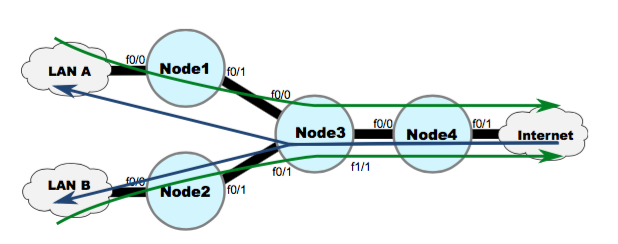
\includegraphics[width=100mm,scale=1]{imagensGuia/ex14.png}
 \label{fig:ex14}
\end{figure}

Neste último exercício pretende-se agora simular o exercício anterior, mas desta vez com tráfego nos dois sentidos, como mostra a imagem acima.

Existem agora quatro tipos de $\lambda$, um para o tráfego que vai da LAN A para a Internet, outro da LAN B para a Internet, e os outros dois da Internet para as LAN's A e B. Foram apenas testados alguns valores, sendo para o tráfego de A para a Internet e da Internet para B utilizou-se 150 e 600. No tráfego da LAN B para a Internet utilizou-se 150 pacotes por segundo e no da Internet para a LAN A, utilizou-se 450. Os valores foram escolhidos de forma a se poder ter vários tipos de amostras diferentes.

No tamanho das filas de espera foram utilizados os mesmos valores do exercício anterior, 64 e 128.

Por último o routing speed e os links podem tomar também os mesmos valores do exercício anterior, 500, 750, 1000 nos routers e 10 Mbits/sec nos links.

Depois de simulado nas mesmas condições do exercício anterior, obtiveram-se os seguintes resultados:

\begin{table}[!htb]
\centering
\resizebox{\textwidth}{!}{\begin{tabular}{lllllllllllllllllll}
\rowcolor[HTML]{FFCC67} 
lambdaAI & lambdaBI & lambdaIA & lamdbaIB & queueSize & B        & R    & Loss Probability nodes & Loss Probability links & Loss Probability & Average Delay ABI & Average Delay IA & Average Delay IB & Transmitted bandwidth ABI & Transmitted bandwidth IA & Transmitted bandwidth IB & WkABI    & WkIA     & WkIB     \\
150      & 150      & 450      & 150      & 64        & 10000000 & 500  & 50.33681               & 0                      & 50.33681         & 0.26196           & 0.26221          & 0.26121          & 136038.92                 & 209406.18                & 70317.12                 & -0.00527 & -0.01019 & -0.0024  \\
150      & 150      & 450      & 150      & 64        & 10000000 & 750  & 19.89152               & 0                      & 19.89152         & 0.16903           & 0.16915          & 0.16874          & 193003.4                  & 292033.42                & 98043.16                 & -0.00666 & -0.00603 & -0.01143 \\
150      & 150      & 450      & 150      & 64        & 10000000 & 1000 & 0                      & 0                      & 0                & 0.01188           & 0.01195          & 0.01154          & 234597.2                  & 353922.36                & 116578.96                & 0.02419  & 0.02418  & 0.0217   \\
150      & 150      & 450      & 150      & 128       & 10000000 & 500  & 50.34569               & 0                      & 50.34569         & 0.51662           & 0.51725          & 0.51634          & 136382                    & 210202.24                & 69967.88                 & -0.00527 & -0.01019 & -0.0024  \\
150      & 150      & 450      & 150      & 128       & 10000000 & 750  & 20.40299               & 0                      & 20.40299         & 0.3382            & 0.33951          & 0.33873          & 163103.46                 & 313569.02                & 102153.64                & -0.00666 & -0.00603 & -0.01143 \\
150      & 150      & 450      & 150      & 128       & 10000000 & 1000 & 0                      & 0                      & 0                & 0.01201           & 0.01205          & 0.01177          & 233225.9                  & 351512.16                & 118515.4                 & 0.02419  & 0.02418  & 0.0217   \\
150      & 150      & 450      & 600      & 64        & 10000000 & 500  & 68.86081               & 0                      & 68.86081         & 0.26375           & 0.26291          & 0.26328          & 96839.9                   & 136728.82                & 181109.86                & -0.00712 & -0.00407 & -0.00167 \\
150      & 150      & 450      & 600      & 64        & 10000000 & 750  & 50.1679                & 0                      & 50.1679          & 0.17415           & 0.17515          & 0.17536          & 60020.2                   & 223501.38                & 302346.2                 & 0.00223  & 0.00209  & -0.00037 \\
150      & 150      & 450      & 600      & 64        & 10000000 & 1000 & 29.5911                & 0                      & 29.5911          & 0.12986           & 0.12944          & 0.12957          & 194264.96                 & 258172.5                 & 344580.34                & -0.00023 & -0.00207 & -0.00046 \\
150      & 150      & 450      & 600      & 128       & 10000000 & 500  & 66.64566               & 0                      & 66.64566         & 0.51748           & 0.51817          & 0.51874          & 36064.9                   & 108654.66                & 146795.44                & -0.00712 & -0.00407 & -0.00167 \\
150      & 150      & 450      & 600      & 128       & 10000000 & 750  & 50.84066               & 0                      & 50.84066         & 0.34399           & 0.3452           & 0.34532          & 75700.36                  & 216002.56                & 286744.34                & 0.00223  & 0.00209  & -0.00037 \\
150      & 150      & 450      & 600      & 128       & 10000000 & 1000 & 31.82792               & 0                      & 31.82792         & 0.25694           & 0.25722          & 0.25737          & 147973                    & 258912.8                 & 348467.82                & -0.00023 & -0.00207 & -0.00046 \\
600      & 150      & 450      & 150      & 64        & 10000000 & 500  & 74.20734               & 0                      & 74.20734         & 0.35814           & 0.38697          & 0.26215          & 104935.18                 & 73365.22                 & 28387.62                 & 0.00049  & -0.00141 & 0.00024  \\
600      & 150      & 450      & 150      & 64        & 10000000 & 750  & 49.68963               & 0                      & 49.68963         & 0.21033           & 0.22679          & 0.17412          & 491713.02                 & 133301.62                & 45330                    & -0.00226 & -0.00353 & -0.00143 \\
600      & 150      & 450      & 150      & 64        & 10000000 & 1000 & 31.99804               & 0                      & 31.99804         & 0.13317           & 0.13402          & 0.12951          & 424488.96                 & 256770.1                 & 86573.1                  & -0.01813 & -0.01841 & -0.00401 \\
600      & 150      & 450      & 150      & 128       & 10000000 & 500  & 76.6031                & 0                      & 76.6031          & 0.71806           & 0.77081          & 0.51775          & 140712.56                 & 114448.36                & 43204.78                 & 0.00049  & -0.00141 & 0.00024  \\
600      & 150      & 450      & 150      & 128       & 10000000 & 750  & 52.50524               & 0                      & 52.50524         & 0.47249           & 0.51126          & 0.34368          & 219673.08                 & 270427.16                & 98557.9                  & -0.00226 & -0.00353 & -0.00143 \\
600      & 150      & 450      & 150      & 128       & 10000000 & 1000 & 32.06684               & 0                      & 32.06684         & 0.26135           & 0.26234          & 0.25726          & 422491.92                 & 258191.26                & 85348.28                 & -0.01813 & -0.01841 & -0.00401 \\
600      & 150      & 450      & 600      & 64        & 10000000 & 500  & 79.66835               & 0                      & 79.66835         & 0.36033           & 0.38739          & 0.26384          & 220319.6                  & 66360.78                 & 144073.14                & -0.0005  & 0.00025  & -0.00086 \\
600      & 150      & 450      & 600      & 64        & 10000000 & 750  & 70.69482               & 0                      & 70.69482         & 0.22593           & 0.23897          & 0.17464          & 126897.84                 & 74710.62                 & 102914.34                & -0.00127 & -0.00076 & 0.00106  \\
600      & 150      & 450      & 600      & 64        & 10000000 & 1000 & 55.3634                & 0                      & 55.3634          & 0.13291           & 0.1334           & 0.13162          & 255797.56                 & 187494.38                & 249237.76                & -0.0144  & -0.0085  & 0.00275  \\
600      & 150      & 450      & 600      & 128       & 10000000 & 500  & 79.58856               & 0                      & 79.58856         & 0.67239           & 0.77029          & 0.51877          & 67990.2                   & 46567.02                 & 103916.74                & -0.0005  & 0.00025  & -0.00086 \\
600      & 150      & 450      & 600      & 128       & 10000000 & 750  & 67.0717                & 0                      & 67.0717          & 0.47176           & 0.50473          & 0.34639          & 110777.72                 & 185365.8                 & 257259.56                & -0.00127 & -0.00076 & 0.00106  \\
600      & 150      & 450      & 600      & 128       & 10000000 & 1000 & 56.31989               & 0                      & 56.31989         & 0.26047           & 0.26055          & 0.25921          & 337029.38                 & 163203.22                & 216796.3                 & -0.0144  & -0.0085  & 0.00275 
\end{tabular}}
\caption[]{Valores teóricos e simulados do atraso e da probabilidade de perda de pacotes utilizando a aproximação de Kleinrock \footnotemark}
\end{table}

\footnotetext{Todos os valores das tabelas são uma média de várias amostras}

Analisando agora os resultados obtidos e mostrados na tabela acima, é possível verificar que apenas não há perdas de pacotes num único caso, quando o routing speed é 1000 pacotes por segundo e a soma dos pacotes num nó nos dois sentidos não ultrapassa esse valor que é o caso em que os valores de $\lambda$ são, 150 no sentido LAN A - Internet, 150 no sentido LAN B - Internet, 450 no sentido Internet - LAN A e 150 no sentido Internet - LAN B.

Note-se ainda que tal como se verificou anteriormente, o cálculo do atraso recorrendo à aproximação de Kleinrock, apenas não falha nos casos onde não há perdas de pacotes. 

Mais uma vez se verifica que não existe perdas de pacotes nos Links, pois estes têm uma largura de banda suficiente para que não se perca nada. Verifica-se ainda que a probabilidade de perdas vai aumentando consoante os valores de $\lambda$, pacotes por segundo, vão aumentando, o que é normal dado os valores de routing speed utilizados, para que os Nodes suportassem, este aumento de pacotes por segundo, seria necessário melhorar o processamento dos routers. Esta solução é válida pois se pode verificar a mesma através da comparação da perda de pacotes para routing speed diferentes.

As fórmulas utilizadas para o cálculo dos atrasos com a aproximação de Kleinrock foram as seguintes:

\[WkABI = \left(\frac{\lambda_{AI}}{\mu_{R} - \lambda_{AI} - \lambda_{IA}}\right) + 
\left(\frac{\lambda_{AI}}{\mu_{L} - \lambda_{AI}}\right) + 
\left(\frac{\lambda_{BI}}{\mu_{R} - \lambda_{BI} - \lambda_{IB}}\right) + 
\left(\frac{\lambda_{BI}}{\mu_{L} - \lambda_{BI}}\right)\] 
\[+ 2 \times \left(\frac{\lambda_{ABI}}{\mu_{R} - \lambda_{ABI} - \lambda_{IBA}}\right) + 2 \times \left(\frac{\lambda_{ABI}}{\mu_{L} - \lambda_{ABI}}\right)\]

\[WkIA = 2 \times \left(\frac{\lambda_{IBA}}{\mu_{R} - \lambda_{IBA} - \lambda_{ABI}}\right) + 
\left(\frac{\lambda_{IBA}}{\mu_{L} - \lambda_{IBA}}\right) + 
 2 \times \left(\frac{\lambda_{IA}}{\mu_{L} - \lambda_{IA}}\right) + \]
\[\left(\frac{\lambda_{IA}}{\mu_{R} - \lambda_{IA} - \lambda_{AI}}\right)\]

\[WkIB = 2 \times \left(\frac{\lambda_{IBA}}{\mu_{R} - \lambda_{IBA} - \lambda_{ABI}}\right) + 
\left(\frac{\lambda_{IBA}}{\mu_{L} - \lambda_{IBA}}\right) + 
 2 \times \left(\frac{\lambda_{IB}}{\mu_{L} - \lambda_{IB}}\right) + \]
\[\left(\frac{\lambda_{IB}}{\mu_{R} - \lambda_{IB} - \lambda_{BI}}\right)\]

A primeira fórmula, calcula o atraso existente, desde as LAN's A e B para a Internet. A única diferença em relação à fórmula utilizada no exercício 13 é que agora no cálculo dos atrasos nos Nodes, tem de se ter em consideração o valor de $\lambda$ que passa no Node no sentido da Internet, e o valor $\lambda$ que passa no sentido das LAN's A e B. Nesta primeira fórmula, calcula-se o atraso nos Nodes, tendo agora em conta o fluxo de pacotes nos dois sentidos e calcula-se ainda os atrasos nos Links. 

A segunda fórmula, corresponde ao atraso existente no fluxo de pacotes desde a Internet para a LAN A. Nos Nodes, continua-se a calcular o atraso tendo em conta os dois sentidos e nos Links calcula-se o atraso normal, pois cada Link é unidirecional.

A terceira e última fórmula é semelhante à anterior, sendo esta referente ao tráfego que vai desde a Internet para a LAN B.

\end{document}



